\begin{itemize}[label=\(\rhd\)]
    \item SQL is based on \textbf{multisets} (or bags) rather than sets. In a multiset an element may occur multiple times.
    \begin{itemize}[label=\(\rhd\)]
        \item Reasons for not automatically removing duplicates:
        \begin{itemize}[label=\(\rhd\)]
            \item expensive to remove duplicates (sorting)
            \item for aggregation duplicates are relevant
        \end{itemize}

    \end{itemize}
    \item We write \{...\} for a set and \{\{...\}\} for a bag
\end{itemize}

\begin{table}[H]
\centering
\begin{tabular}{|c|c|c|}
    \specialrule{0.01em}{0em}{0em} 
     \textbf{SQL} & \textbf{Relational Algebra} & \textbf{Domain Relational Calculus}  \\
    \specialrule{0.01em}{0em}{0em} 
     table & relation & predicate \\
    \specialrule{0.005em}{0em}{0em} % Fine line with specified thickness and spacing
     column & attribute & argument\\
    \specialrule{0.005em}{0em}{0em}  % Fine line with specified thickness and spacing
    row & tuple & - \\
    \specialrule{0.005em}{0em}{0em}  % Fine line with specified thickness and spacing
    query & RA expression & formula \\
     \specialrule{0.01em}{0em}{0em} 
\end{tabular}
\end{table}

\subsection{Data Definition Language}

\subsubsection{Domain Types}
Domain Types in SQL:
\begin{itemize}[label=\(\rhd\)]
    \item CHAR(n): fixed length character string
    \item VARCHAR(n): character string with maximum length $n$
    \item INTEGER
    \item SMALLINT
    \item NUMERIC(p,d): Fixed point number, user-specified precision of $p$ digits, with $n$ digits to the right of decimal point
    \item REAL, DOUBLE PRECISION: Floating point and double-precision floating point numbers
    \item FLOAT(n): Floating point number, with user-specified precision of at least $n$ digits
\end{itemize}
\subsubsection{Create, dropping and altering tables}
\textbf{\underline{Create Table Construct}}
\bigskip

Example: 
\begin{lstlisting}[caption= Create Table Example]
    CREATE TABLE branch (
        BranchName CHAR(15),
        BranchCity CHAR(30),
        Assets INTEGER )
\end{lstlisting}

\textbf{\underline{Drop and Alter Table Constructs}}
\bigskip
\begin{itemize}[label=\(\rhd\)]
    \item The \textbf{drop table} command deletes the whole table from the database
    \item The \textbf{alter table} command is used to add columns to an existing table
    \begin{itemize}[label=\(\rhd\)]
        \item[] \textbf{alter table} r \textbf{add} $A$ $D$ 
    \end{itemize}
\end{itemize}


\subsubsection{Integrity constrains}

\begin{itemize}[label=\(\rhd\)]
    \item Integrity constraints guard against damage to the database
    \item Formally, an integrity constraint is a closed first order formula that must be true, i.e., that each database instance must satisfy.
    \begin{itemize}[label=\(\rhd\)]
        \item Example: $\forall B(account(\_,\_,B) \Rightarrow B<10M)$
    \end{itemize}
\end{itemize}

Integrity constraints on single relations:
\begin{itemize}[label=\(\rhd\)]
    \item \textbf{Domain Constraints}
    \begin{itemize}[label=\(\rhd\)]
        \item Domain constraints are the most elementary form of integrity constraints. They check values inserted in the database, and they check queries to ensure that the comparisons make sense.
        \item New domains can be created from existing data types
        \item Example:
        \begin{itemize}[label=\(\rhd\)]
            \item[] \begin{lstlisting}
                CREATE DOMAIN Dollars INTEGER
                CREATE DOMAIN Pounds INTEGER
            \end{lstlisting}
        \end{itemize}
        \item We cannot assign or compare a value of type Dollar to a value of type Pounds. But we can convert values: 
        \begin{itemize}[label=\(\rhd\)]
            \item[] \begin{lstlisting}
                CAST(r.Amnt/1.5 AS Pounds)
            \end{lstlisting}
        \end{itemize}
    \end{itemize}
    \item \textbf{not null}
    \begin{itemize}[label=\(\rhd\)]
        \item[] \begin{lstlisting}
            BranchName VARCHAR(15) NOT NULL
            CREATE DOMAIN Dollars INTEGER NOT NULL
        \end{lstlisting}
    \end{itemize}
    \item \textbf{primary key}
    \begin{itemize}[label=\(\rhd\)]
        \item A primary key ensures that an attribute value is not null and unique across all rows of a table. Therefore it can be used to identify a unique row in a table, and is used for query optimization
        \item Within the Create Table construct include \begin{lstlisting}
            PRIMARY KEY (CustName)
        \end{lstlisting}
    \end{itemize}
    \item \textbf{unique}
    \begin{itemize}[label=\(\rhd\)]
        \item The unique specification states that the attributes $A_1,A_2,...,A_m$ form a candidate key.
        \item Candidate keys are permitted to be null 
    \end{itemize}
    \item \textbf{check}($P$), where $P$ is a predicate over a single relation 
    \begin{itemize}[label=\(\rhd\)]
        \item Within the Create Table Construct include: \begin{lstlisting}
            CHECK (Assets >= 0)
        \end{lstlisting}
    \end{itemize}
\end{itemize}

Integrity constraints over multiple relations (Referential Integrity):
\begin{itemize}[label=\(\rhd\)]
    \item \textbf{foreign key}
    \begin{itemize}[label=\(\rhd\)]
        \item Within the Create Table Construct include:
        \begin{lstlisting}
            FOREIGN KEY (BranchN) REFERENCES branch
        \end{lstlisting}
    \end{itemize}
    \item \textbf{check}($P$), where $P$ is a predicate over multiple relations
    \item \textbf{assertion}
    \begin{itemize}[label=\(\rhd\)]
        \item An assertion is a predicate expressing a condition that the database must satisfy.
        \item An assertion in SQL takes the form
        \begin{itemize}[label=\(\rhd\)]
            \item[] \textbf{create assertion} <assertion-name> \textbf{check} <predicate>
        \end{itemize}
    \end{itemize}
\end{itemize}
\subsection{Expressions and Predicates}
\textbf{\underline{Expressions}}
\bigskip

\begin{itemize}[label=\(\rhd\)]
    \item Numeric functions: $+,-,*,/, abs(e), ceil(e), tan(e), log(e), round(e), sign(e), mod(e,f),...$
    \item Character functions:
    \begin{itemize}[label=\(\rhd\)]
        \item concatenation: 'abc' || 'de' = 'abcde'
        \item \textbf{position}('48' \textbf{in} 'another 48 hours') = 9
        \item \textbf{substring}('anothe' \textbf{from} 1 \textbf{for} 3) = 'ano'
        \item \textbf{upper}(e)
        \item \textbf{trim}(\textbf{leading} ' ' \textbf{from} ' test') = 'test
    \end{itemize}
    \item date and time functions:
    \begin{itemize}[label=\(\rhd\)]
        \item \textbf{current\_date}, \textbf{current\_time}
        \item \textbf{current\_timestamp}
        \item \textbf{current\_date} + \textbf{interval} '1' \textbf{day}
        \item \textbf{current\_date} - \textbf{date} '1990/3/18'
        \item \textbf{interval} '6' \textbf{day} - \textbf{interval} 'a' \textbf{day} = \textbf{interval} '5' \textbf{day}
     \end{itemize}
     \item type conversions:
     \begin{itemize}[label=\(\rhd\)]
         \item \textbf{cast}('48' \textbf{as integer}) = 48
         \item often "natural" type conversions are done implicitly
     \end{itemize}
     \item conditional statement:
     \begin{lstlisting}
         case
         when cond1 then result1
         ...
         when condN then resultN
         else resultX
         end
     \end{lstlisting}
     \item \textbf{coalesce}(val1,..., valN)
     \begin{itemize}[label=\(\rhd\)]
         \item returns the first value that is not null (and null if all values are equal to null)
     \end{itemize}
     \item  \textbf{nullif}(e1,e2)
     \begin{itemize}[label=\(\rhd\)]
         \item returns null if e1 and e2 are identical; useful if missing information is not represented with null; \textbf{nullif}(cost,9999)
     \end{itemize}
\end{itemize}

\textbf{\underline{Predicates}}
\bigskip

\begin{itemize}[label=\(\rhd\)]
    \item Predicates evaluate to true, false or unknown
    \item boolean connectives: \textbf{and}, \textbf{or}, \textbf{not}
    \item $=,<>, <,>,<=,>=$
    \item e \textbf{[not] between} e1 \textbf{and} e2
    \item e \textbf{is [not] null}
    \item e \textbf{in} (e1,...,eN)
    \item e1 \textbf{like} e2
    \begin{itemize}[label=\(\rhd\)]
        \item example:
        \begin{lstlisting}
            Name like '_ross%'
        \end{lstlisting}
        \item wildcards: \% 0-n characters, \_ 1 character
    \end{itemize}
\end{itemize}



\subsection{Table Expressions, Query Specifications, Query Expressions}
\textbf{\underline{Structure of SQL Queries:}}
\bigskip

\begin{figure}[H]
\centering
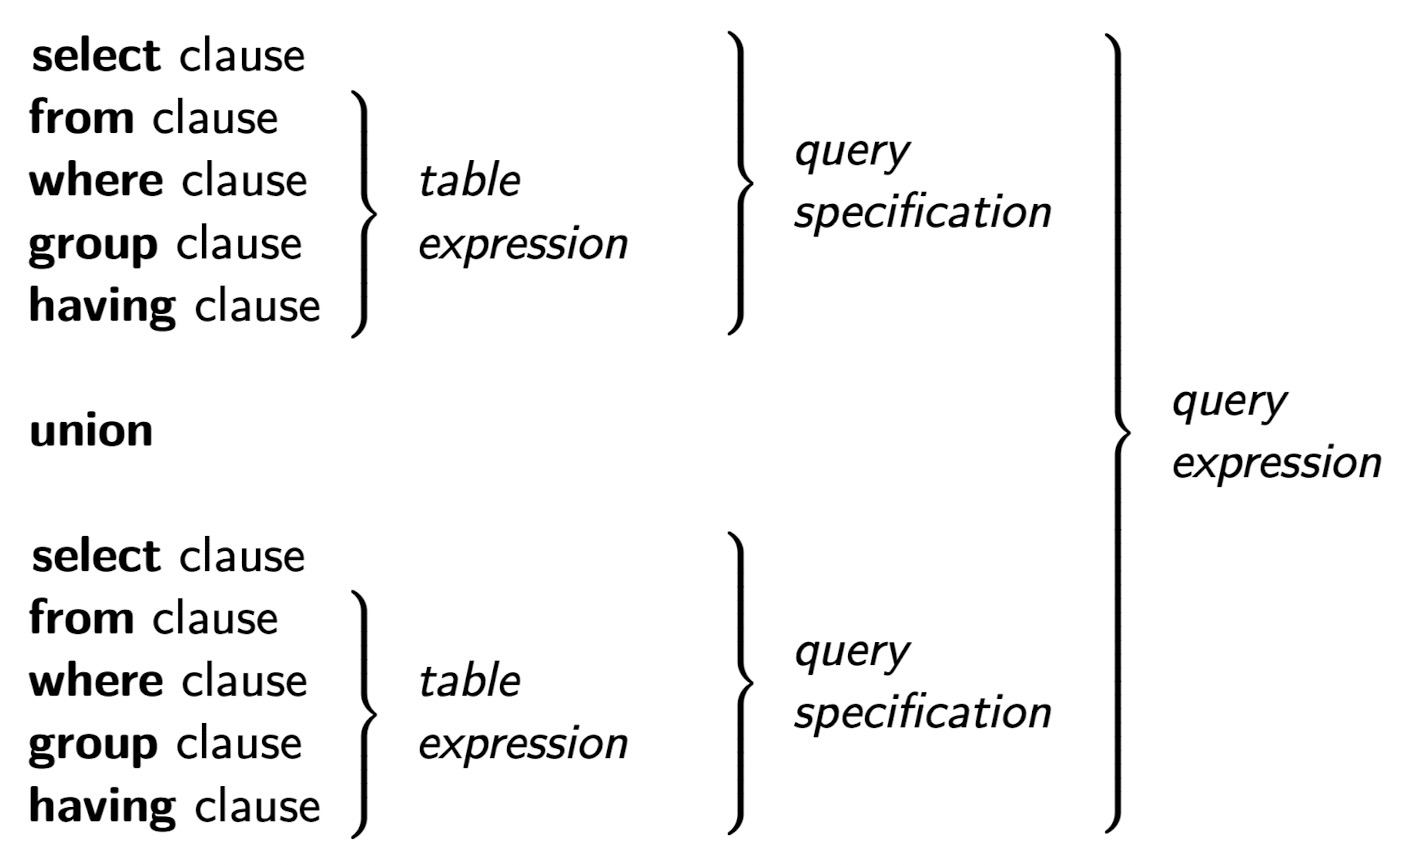
\includegraphics[width=0.6\textwidth]{images/Screenshot 2024-05-04 at 16.56.14.jpg}
\caption{SQL Structure}
\end{figure}

The result of an SQL query is a (virtual) table.

\subsubsection{The from Clause}

\begin{itemize}[label=\(\rhd\)]
    \item The \textbf{from} clause lists the table involved in the query
    \begin{itemize}[label=\(\rhd\)]
        \item Corresponds to the Cartesian product operation of the relational algebra (if multiple tables listed in from clause)
    \end{itemize}
    \item Many different joins supported
    \begin{itemize}[label=\(\rhd\)]
        \item \textbf{CROSS JOIN} = Cartesian product (implicitly also given without keyword)
        \item \textbf{Theta Join}: \quad \textbf{FROM} t1 \textbf{JOIN} t2 \textbf{ON} t1.a < t2.b
        \item \textbf{Left Outer Join}: \quad \textbf{FROM} t1 \textbf{LEFT OUTER JOIN} t2 \textbf{ON} t1.a = t2.b
        \item \textbf{Natural Join}:  \quad \textbf{FROM} t1 \textbf{NATURAL INNER JOIN} t2 
        \item \textbf{Limited Natural Join} (not all pair-wise equal columns are used for the natural join; only the ones specified in the using clause):  \quad \textbf{FROM} t1 \textbf{NATURAL INNER JOIN} t2 \textbf{USING} (name)
    \end{itemize}
\end{itemize}

\subsubsection{The where Clause}

\begin{itemize}[label=\(\rhd\)]
    \item The \textbf{where} clause specifies conditions that the result tuples must satisfy
    \item Example:
    \begin{lstlisting}
        FROM loan
        WHERE BranchName = 'Perryridge' 
            AND Amount > 1200
    \end{lstlisting}
    \item logical connectives: and, or, not
\end{itemize}

\subsubsection{The group Clause}
\begin{itemize}[label=\(\rhd\)]
    \item The \textbf{group} clause takes the table produced by the where clause and returns a grouped table
    \item Example:
    \begin{lstlisting}
        FROM account
        GROUP BY BranchName
    \end{lstlisting}
    \item The following statements work on the groups (and not on individual tuples)
\end{itemize}

\subsubsection{The having Clause}
\begin{itemize}[label=\(\rhd\)]
    \item The \textbf{having} clause takes a grouped table as input and returns a grouped table
    \item The having condition is applied to each group. Only groups that satisfy it are returned
    \item Example:
    \begin{lstlisting}
        FROM account
        GROUP BY BranchName
        HAVING COUNT(AccNr) > 1
    \end{lstlisting}
\end{itemize}

\subsubsection{The select Clause}
\begin{itemize}[label=\(\rhd\)]
    \item The \textbf{select} clause lists the columns that shall be in the result of a query
    \begin{itemize}[label=\(\rhd\)]
        \item Corresponds to the projection operation of RA
    \end{itemize}
    \item To force the elimination of duplicates, insert the keyword \textbf{distinct} after select
    \item In the select clause aggregate functions can be used:
    \begin{itemize}[label=\(\rhd\)]
        \item avg, min, max, sum, count
    \end{itemize}
\end{itemize}

\subsubsection{Derived Tables}
\begin{itemize}[label=\(\rhd\)]
    \item SQL allows a query expression to be used in the \textbf{from} clause
    \item Example:
    \begin{lstlisting}
        SELECT BranchName, AvgBalance
        FROM ( SELECT BranchName AVG(Balance)
               FROM account
               GROUP BY BranchName
             ) AS branchAvg(BranchName, AvgBalance)
        WHERE AvgBalance > 1200
    \end{lstlisting}
\end{itemize}

\subsubsection{Query Expressions}
\begin{itemize}[label=\(\rhd\)]
    \item The set operations \textbf{union}, \textbf{intersect}, and \textbf{except} operate on tables and correspond to the relational algebra operations $\cup, \cap, -$
    \item Each automatically removes duplicates, to preserve duplicates add \textbf{all} after operator
\end{itemize}

\subsection{Subqueries, Duplicates, Null Values}

\subsubsection{Subqueries}

\begin{itemize}[label=\(\rhd\)]
    \item A \textbf{subquery} is a \textbf{query expression} that is nested within another query expression.
    \item Example:
    \begin{lstlisting}
        SELECT X FROM p WHERE X IN (SELECT Y FROM q)
    \end{lstlisting}
    \item[\textbf{!}] Semantics/evaluation: For each tuple of p evaluate the subquery and check if X is in the result table computed by the subquery
    \item The \textbf{exists} construct returns the value \textbf{true} if the argument subquery is nonempty
    \begin{itemize}[label=\(\rhd\)]
        \item[\textbf{!}] Use \textbf{exists} instead of \textbf{in, all, any, some}
    \end{itemize}
\end{itemize}

\subsubsection{Duplicates}

SQL duplicate semantics:\\

\quad \textbf{select} $A_1,A_2,...,A_n$ \

\quad \textbf{from} $r_1, r_2,...,r_m$ \

\quad \textbf{where} $P$\\

is equivalent to the \textit{multiset} version of the expression: \[
\pi_{A_1,A_2,...,A_n}(\sigma_P (r_1 \times r_2 \times ... \times r_m))
\]

\subsubsection{Null Values}
\begin{itemize}[label=\(\rhd\)]
    \item The  predicate \textbf{is null} can be used to check for null values.
    \item Any comparison with \textit{null} returns unknown
    \begin{itemize}[label=\(\rhd\)]
        \item Example: $5<null$ or $null<>null$ or $null=null$ 
    \end{itemize}
    \item All aggregate operations, expect \textbf{count(*)}, ignore tuples with null values on the aggregated columns. 
    \begin{itemize}[label=\(\rhd\)]
        \item Arithmetic operations like $7+ null = null$, thus they do not ignore null values
    \end{itemize}
\end{itemize}

\subsubsection{Ordering}

\begin{itemize}[label=\(\rhd\)]
    \item \textbf{ORDER BY} CustName => orders the result table alphabetically (ascending = default)
    \item \textbf{ORDER BY} CustName \textbf{DESC} => in descending order
\end{itemize}

\subsection{Modification of the Database}

\subsubsection{Insertions}
\begin{lstlisting}
    INSERT INTO account
        VALUES ('A-9732', 'Perryridge', 1200)
\end{lstlisting}

\subsubsection{Deletions}
\begin{lstlisting}
    DELETE FROM account
    WHERE BranchName = 'Perryridge'
\end{lstlisting}
\subsubsection{Updates}
\begin{lstlisting}
    UPDATE account
    SET Balance = Balance * 1.06
    WHERE Balance > 10000

    UPDATE account 
    SET Balance = Balance * 1.05
    WHERE Balance <= 10000
\end{lstlisting}
Here order matters! $\Rightarrow$ Better use the \textbf{case} statement 
\begin{lstlisting}
    UPDATE account
    SET Balance = CASE 
                    WHEN Balance <= 10000
                    THEN Balance * 1.05
                    ELSE Balance * 1.06
                  END
\end{lstlisting}   

\subsection{Views}


\subsubsection{Purpose of views}

\begin{itemize}[label=\(\rhd\)]
    \item A view is a table whose rows are not stored in the database. The rows are computed when needed from the view definition.
    \item A view provides a mechanism to hide data from the view of users, or to give users direct access to the results of (complex) computations.
\end{itemize}
\subsubsection{Creation and use of views}

\begin{itemize}[label=\(\rhd\)]
    \item A view is defined using the \textbf{create view} statement which has the form 
    \begin{itemize}[label=\(\rhd\)]
        \item[] \textbf{CREATE VIEW} \textit{v} \textbf{AS} <query expression>
    \end{itemize}
\end{itemize}

\subsubsection{Handling views in the DBMS}
\begin{itemize}[label=\(\rhd\)]
    \item The view definition is stored in the meta database.
    \item A view is \textbf{updatable} if the database system can determine the reverse mapping 
    \item Example:
    \begin{itemize}[label=\(\rhd\)]
        \item[] \begin{lstlisting}
            CREATE VIEW goodStudents (sid, gpa) AS
                SELECT SID, GPA
                FROM students
                WHERE GPA > 3.0;

            INSERT INTO goodStudents VALUES (51234, 2.8)                 
        \end{lstlisting}
        \begin{itemize}[label=\(\rhd\)]
            \item Result: student is inserted into students relation, but cannot be retrieved through the view \textit{goodStudents}
        \end{itemize}
    \end{itemize}
\end{itemize}

\subsubsection{Temporary Views - With Clause}
\begin{itemize}[label=\(\rhd\)]
    \item The \textbf{with} clause provides a way of defining temporary views whose definition is only available to the query in which the \textbf{with} clause occurs
    \item Example:
    \item[] \begin{lstlisting}
        WITH
        maxBalance (Val) AS (
            SELECT MAX(Balance)
            FROM account
        )
        SELECT AccNr
        FROM account, maxBalance
        WHERE account.Balance = maxBalance.Val
    \end{lstlisting}
\end{itemize}

\subsubsection{Recursion in SQL}
\begin{itemize}[label=\(\rhd\)]
    \item Recursive views are required to be \textbf{monotonic}. That is, if we add tuples to \textit{manager} the view contains all of the tuples it contained before, plus possibly more.
    \item Example:
    \begin{itemize}[label=\(\rhd\)]
        \item[] \begin{lstlisting}
            WITH RECURSIVE mgr(EmpName, MgrName) AS (
                SELECT EmpName, BossName % base case
                FROM empl
                UNION
                SELECT empl.EmpName, mgr.MgrName % recursive case
                FROM empl, mgr
                WHERE BossName = mgr.EmpName
            )
            SELECT * FROM mgr;
        \end{lstlisting}
        \item View \textit{mgr} is the \textbf{transitive closure} of the \textit{empl} relation
    \end{itemize}
\end{itemize}


\subsection{User Defined Functions (UDF)}
\begin{itemize}[label=\(\rhd\)]
    \item User defined functions or stored procedures allow to execute application logic in the process space of the DBMS.
    \item $\Rightarrow$ good for performance since it reduces the amount of data that is transferred between client and server.
\end{itemize}

\subsubsection{PL/pgSQL value functions}
\begin{itemize}[label=\(\rhd\)]
    \item Structure
    \begin{lstlisting}[]
        create function somefunc()
        returns < retype > as $$
        [ declare 
            < declarations> ]
        begin 
            < statements >
        end;
        $$ language plpgsql;
    \end{lstlisting}
    \item < \textit{retype} >
        \begin{itemize}[label=\(\rhd\)]
            \item INTEGER, RECORD, TABLE, ...
        \end{itemize}
    \item < \textit{declarations} >
    \begin{lstlisting}
        quantity INTEGER := 30;
        tbl_row account%ROWTYPE;
    \end{lstlisting}
    \item < \textit{statements} >
    \begin{lstlisting}
        quantity := 4;

        IF quantity < 5 THEN
            quantity := 5;
        END IF;

        WHILE quantity < 10 LOOP
            quantity := quantity + 1;
        END LOOP;     
    \end{lstlisting}
    \item A \textbf{value function} returns a value (or tuple) 
    \item Example:
    \begin{lstlisting}
        CREATE FUNCTION accountCnt (CName VARCHAR(9))
        RETURNS INTEGER AS
        $$
        DECLARE
            accCnt INTEGER;
        BEGIN 
            SELECT COUNT(*) INTO accCnt
            FROM depositor
            WHERE depositor.CustName = CName;
            RETURN accCnt;
        END;
        $$ LANGUAGE PLPGSQL;
    \end{lstlisting}
    \item Usage: \begin{lstlisting}
        SELECT accountCnt('Bob');
    \end{lstlisting}
\end{itemize}

\subsubsection{PL/pgSQL table functions}
\begin{itemize}[label=\(\rhd\)]
    \item \textbf{Table functions} return a table
    \item Example - All accounts with a balance above a threshold:
    \begin{lstlisting}
        CREATE FUNCTION highAccnts (limitVal INTEGER)
        RETURNS TABLE (AccNum INTEGER,
                       BrName VARCHAR(15),
                       Bal INTEGER) AS
        $$
        BEGIN
            RETURN QUERY
                SELECT AccNr, BranchName, Balance
                FROM account A
                WHERE A.Balance > highAccnts.limitVal;
        END;
        $$ LANGUAGE PLPGSQL;
    \end{lstlisting}
    \item Usage:
    \begin{lstlisting}
        SELECT * FROM highAccnts(1000);
    \end{lstlisting}
\end{itemize}

\subsection{Summary}
\begin{itemize}[label=\(\rhd\)]
    \item DDL (data definition language)
    \begin{itemize}[label=\(\rhd\)]
        \item Used to \textbf{create, alter}, and \textbf{drop} tables.
        \item Table definitions include \textbf{constraints} (domain, not null, primary key, foreign key)
        \item Constraints ensure \textbf{data quality}, which in turn gives competitive advantages to businesses
        \item Enforcing constraints is difficult and requires a focused effort. People try to work around
        \item Data quality must be considered during data acquisition; the database system must enforce it; it cannot be fixed later
    \end{itemize}
    \item Expressions and predicates
    \begin{itemize}[label=\(\rhd\)]
        \item Database systems have been conservative since the efficient evaluation must be considered
        \item The brute force evaluation of a condition on one billion tuples might not be good enough.
        \item Modern database systems are extensible with user defined functions
    \end{itemize}
    \item SQL
    \begin{itemize}[label=\(\rhd\)]
        \item SQL is used very heavily in practice
        \item The building block of the DML are \textbf{query specifications} and \textbf{query expressions}
        \item SQL is more than simple select-from-where. The set based semantics of SQL requires some practice
        \item Know the \textbf{conceptual evaluation}/semantics of query expressions
        \begin{itemize}[label=\(\rhd\)]
            \item From the cross product of the tables in the from clause
            \item Eliminate tuples that do not satisfy the where clause
            \item Group the remaining tuples according to the group clause
            \item Eliminate groups that do not satisfy the having clause
            \item With aggregation one result tuple is produced for each group
            \item Eliminate duplicates if distinct is specified
            \item Compute query expressions independently and apply set operations (union, except, intersect)
            \item Sort all result tuples if order clause is specified
        \end{itemize}
    \end{itemize}
    \item The difference between \textbf{set} and \textbf{multisets} (or bags) is relevant
    \item \textbf{Subqueries} are natural and help understanding: it is possible (and advisable) to only use \textbf{exists} and \textbf{not exists}
    \item Large parts of RA, SQL and DRC are equivalent; know how to go from one to the other
    \item Modification statements use the \textbf{logical update semantics} (compute changes before they are applied)
    \item The SQL OLAP extensions further extend SQL to better support report generation (cross tabs, moving averages, etc.)
    \item \textbf{Views} are essential to break up large tasks (SQL statements) in small, independent and manageable blocks
    \item \textbf{Recursive queries} are used to compute ancestors, descendants, transitive closures, etc.
    \item \textbf{Functions} and \textbf{procedural constructs} are used heavily by many applications
\end{itemize}
